\documentclass{article}

\usepackage[final]{neurips_2019}

\usepackage[utf8]{inputenc}
\usepackage[T1]{fontenc}
\usepackage{hyperref}
\usepackage{url}
\usepackage{booktabs}
\usepackage{amsfonts}
\usepackage{nicefrac}
\usepackage{microtype}
\usepackage{graphicx}
\usepackage{xcolor}
\usepackage{lipsum}

\newcommand{\note}[1]{\textcolor{blue}{{#1}}}

\title{
  Whiskey GPTaster \\
  \vspace{1em}
  \small{\normalfont Stanford CS224N Custom Project}  % Select one and delete the other
}

\author{
  Akram Sbaih \\
  Department of Computer Science \\
  Stanford University \\
  \texttt{akram@stanford.edu} \\
  % Examples of more authors
   \And
   \texttt{Mentor} John Hewitt \\
   Department of Computer Science \\
   Stanford University \\
   \texttt{johnhew@stanford.edu} \\
%   \And
%   Name \\
%   Department of Computer Science \\
%   Stanford University \\
%   \texttt{name@stanford.edu}
}

\begin{document}

\maketitle

\begin{abstract}
%  Your abstract should motivate the problem, describe your goals, and highlight your main findings. Given that your project is still in progress, it is okay if your findings are what you are still working on.
Recent advances in language modeling and text generation started raising concerns on the potential for machines to generate fake news and reviews. These models now generate text shown to be indistinguishable from human text \cite{adelani2019generating}. Some recent approachs \cite{zellers2020defending} train classifiers to discriminate fake and real text. These usually require access to the generator or its training data which aren't usually available in the wild. We're also faced with the constraint of having few examples of identifiable good fakes. In this work, I study the performance of classifiers with combinations of [the generator, its training data, its generations]. To this end, I generated a set of fake whiskey reviews using GPT2 to evaluate these approachs.
\end{abstract}


%\section{Key Information to include}
%\begin{itemize}
%    \item External collaborators (if you have any):
%    \item External mentor (if you have any):
%    \item Sharing project:
%\end{itemize}

% {\color{red} This template does not contain the full instruction set for this assignment; please refer back to the milestone instructions PDF.}

\section{Approach}
%This section details your approach to the problem. 
%\begin{itemize}
%    \item Please be specific when describing your main approaches. You may want to include key equations and figures (though it is fine if you want to defer creating time-consuming figures until the final report).
%    \item Describe your baselines. Depending on space constraints and how standard your baseline is, you might do this in detail or simply refer to other papers for details. Default project teams can do the latter when describing the provided baseline model.
%    \item If any part of your approach is original, make it clear. For models and techniques that are not yours, provide references.
%    \item If you are using any code that you did not write yourself, make it clear and provide a reference or link. 
%    When describing something you coded yourself, make it clear.
%\end{itemize} 
The goal is to make a classifier that takes in a Whiskey review alongside its metadata (price, rating, and name) and decides whether it's human generated or machine generated.  In this project, I define a human-generated review as one that has been scraped from a crowdsourced dataset, while a machine-generated review is one made by GPT2 finetuned on that human dataset. These definitions reflect only a small combination of the potential samples in the wild, but still serve as a good evaluation since GPT2 is one of the widely-used architectures in the market. To this end, there are multiple approaches that I would like to compare. 
\begin{itemize}
\item Finetune GPT2 to be a classifier that takes these input as a sequence and outputs a token deciding whether the review is real or fake, starting from a publicly available GPT2 checkpoint.
\item Finetune GPT2 as the previous approach but start from the checkpoint that was used for generation similar to the approach proposed in \cite{zellers2020defending}.
\item Compare the preplexities on the real and generated sequences for both the public and generator-finetuned checkpoints of GPT2 and train a classifier on those preplexities if necessary. 
\end{itemize}
We should expect that all three approaches perform well. However, each of them offers a different set of constraints. For example, we probably will not have access to the finetuned generator in the wild. We also might be faced with a very limited number of fake reviews from the same generator that we can train a classifier on. Therefore, comparing the results of these approaches offers a valuable understanding of what we can and cannot do to combat bad use of language models for generating fake reviews.
\\ To evaluate these approaches, I set the following milestones
\begin{enumerate}
\item Prepare a dataset of human-generated reviews with their metadata.
\item Finetune Huggingface GPT2 on that dataset to generate novel fake reviews making a new fake-reviews dataset.
\item Implement each of the approaches and assess their accuracy.
\end{enumerate}

\section{Experiments}
%This section is expected to contain the following.
%\begin{itemize}
%    \item \textbf{Data}: Describe the dataset(s) you are using along with references. Make sure the task associated with the dataset is clearly described.
%    \item \textbf{Evaluation method}: Describe the evaluation metric(s) you used, plus any other details necessary to understand your evaluation.
%    \item \textbf{Experimental details}: Please explain how you ran your experiments (e.g. model configurations, learning rate, training time, etc.).
%    \item \textbf{Results}: Report the quantitative results that you have so far. Use a table or plot to compare multiple results and compare against your baselines.
%\end{itemize}
\paragraph{Data}$ $
\\ \href{www.whiskyadvocate.com}{www.whiskyadvocate.com} is a website where people write their reviews and ratings for various whiskeys. I made a script that scraped all the reviews on the website totaling 5649 unique ones. Each review contains the name of the whiskey, its price in dollars, its rating out of 100, and the text review of its taste.  Some examples are shown in Table \ref{reviewstable}. 
\\ I split the data into train, validation, and test sets being 90\%, 6\%, and 4\% which are 5084, 339, and 226 samples, respectively. I intended for the training split to be bigger than the convention because of the limited number of total samples. The test split is also small because main evaluation done on it will be qualitative which is labor-intensive. 
\\ The reviews are reformatted as sequences to be fed into GPT2. An example of the formatting I used is \texttt{"<price>105<rating>89<whiskey>Springbank 11 year old, 58\%<review>Finished in a rum cask. Gently sweet [...] exclusive.)"} where \texttt{[...]} indicates omitted text.

\paragraph{Evaluation method}$ $
\begin{enumerate}
\item Preplexity. This is the average uncertainity the language model has over the sequence it's evaluated on (the lower the better). Since GPT2 is a language model, I used this metric to track how well it's adapting to the new task of modeling whiskey reviews during finetuning. It's also a measure of how well the the final model performs.
\item Qualitative assessment. Since I don't have access to enough labor-work to turn human assessment of the generations into a quantative measure like in \cite{adelani2019generating}, I resorted to my personal assessment. This involves looking at the generated samples for common themes in whiskey reviews. This includes things like having a description of common flavors, distinction between nose and palate, having an after-tast, and mentioning the name of the whiskey in the review. 
\item Accuracy. This is useful for the classifiers proposed in the approach section.
\end{enumerate}

\paragraph{Experimental details}$ $
\\ After preprocessing the dataset, I ran the Huggingface GPT2 Trainer on the training and validation splits for 5 epochs starting with their publicly available pre-trained GPT2 checkpoint. I chose a batch size of 2 per device beecause of the limited available memory. Each sample in the batch is the sequence concatenation of multiple samples from the training set so that we use up all the available GPT2 block size and train faster. 
\\ I trained on an Azure machine with two K-80's making a total batch size of 4 with 4 dataloading workers. I used the default learning rate of $5e-5$ and the default Cross Entropy loss function. Training took 31 minutes and ended up with a preplexity of 15.49 on the validation set.  You can see the loss curve in Figure \ref{Fig:get_finetune_loss_fig}.

\paragraph{Results}$ $
\\The baseline for the generation task is the human generated text since we're not comparing the model to other models because that's not the goal of this project. I use my human evaluation to look for common patterns in the generated text as mentioned in the Evaluation Method section.  The generations seem satisfying except for an observation that the model tends to list too many flavors sometimes. Table \ref{reviewstable} shows a few randomly selected generations from the test set.

\section{Future work}$ $
At this point, I finished the first step of generating the fake reviews dataset and evaluating it. Next, I need to do the following:
\begin{enumerate}
\item Implement and train classifiers proposed in the Approach section.
\item Gather statistics on the performance of these classifiers and their usability in the wild and what constraints they require.
\item Engage more into the ethics of the fake reviews problem and the philosophy of its constraints in the wild.
\end{enumerate}

\begin{figure}[tb]
 \centering
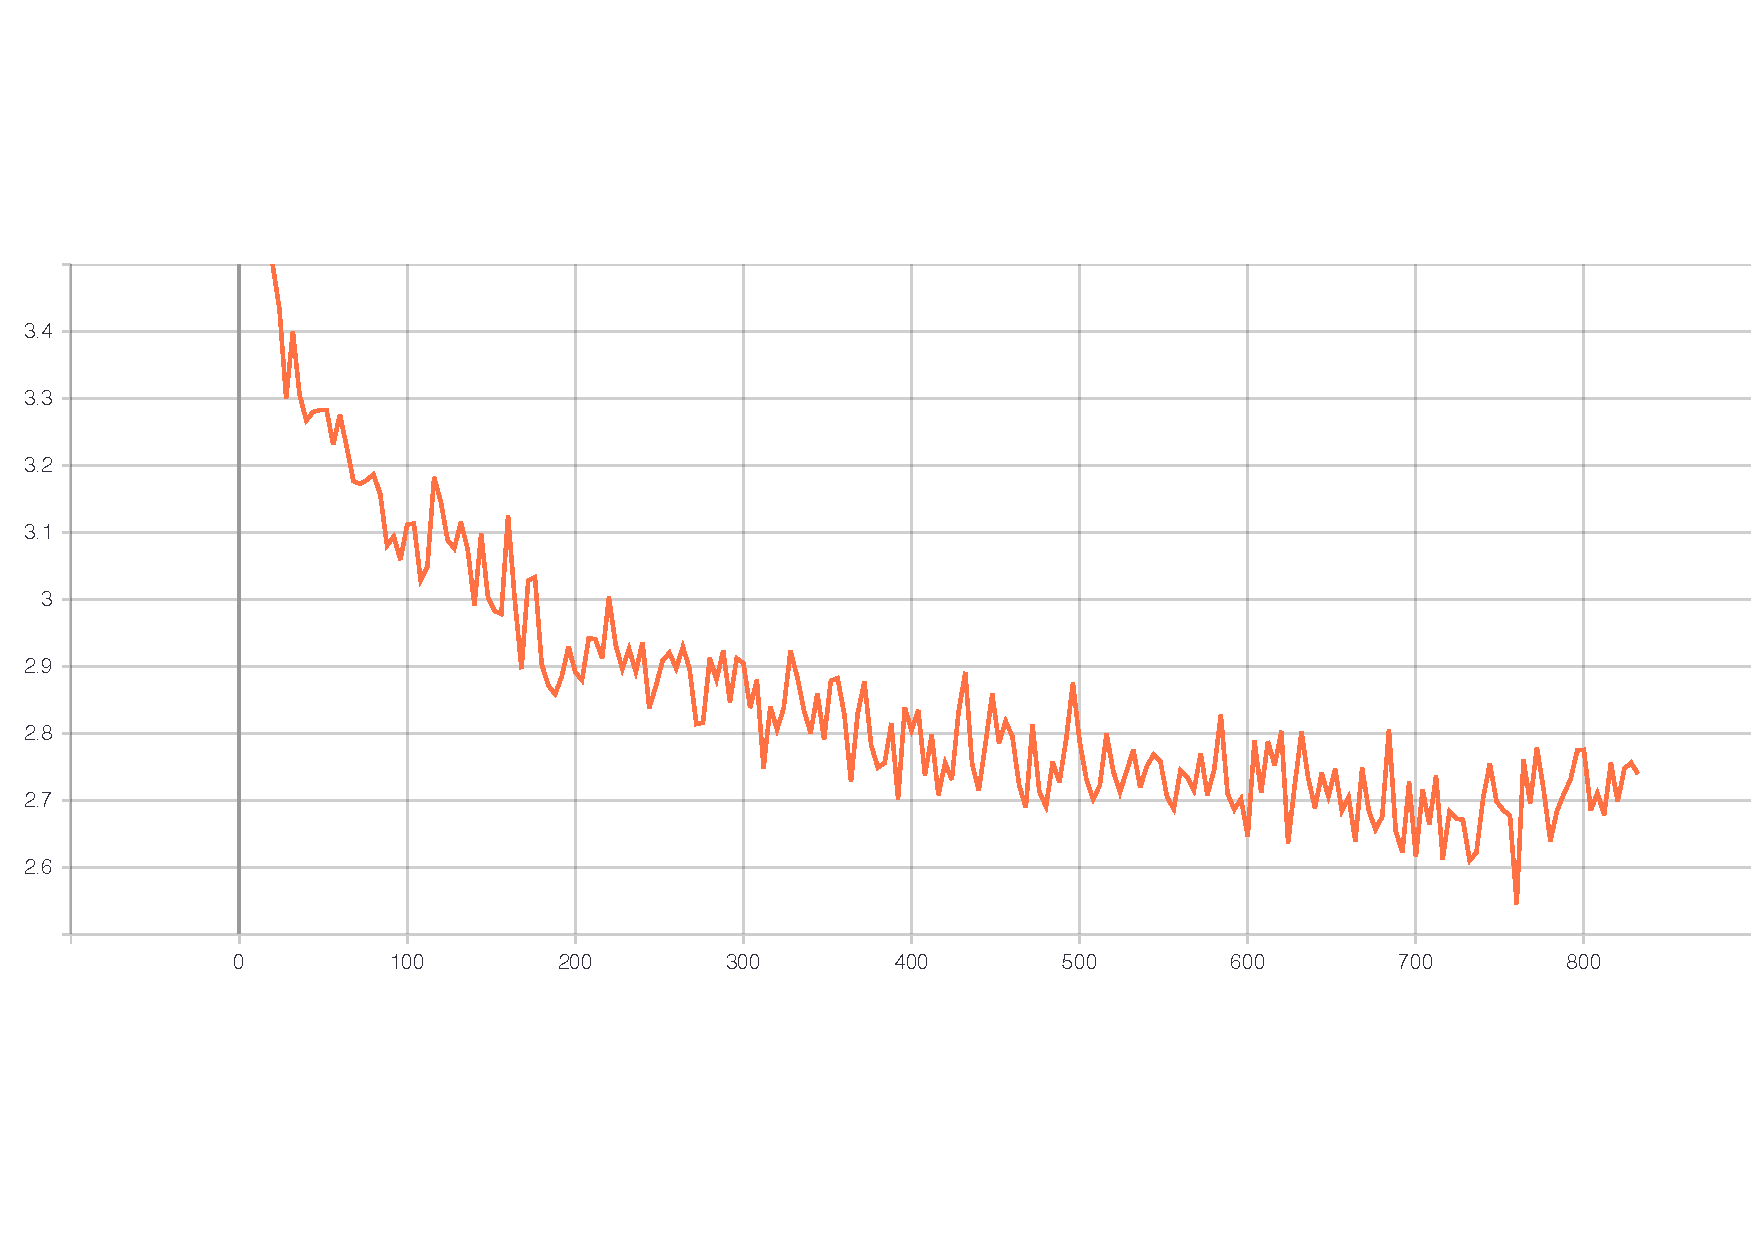
\includegraphics[width=0.7\columnwidth]{finetune_condgen_train_loss.pdf}
\vspace{-4mm}
\caption{GPT2 Training Loss for 5 epochs.}
\label{Fig:get_finetune_loss_fig}
\vspace{-3mm}
\end{figure}

\begin{table}[h]
    \centering
    \begin{tabular}{p{0.45\linewidth} | p{0.45\linewidth}}
        \toprule
        \textbf{Real} & \textbf{Fake} \\
        \midrule
        <price>495<rating>89<whiskey>Bainbridge Yama American Single Grain Barley Mizunara Japanese Oak Cask, 45\%<review>This high-end whiskey exhibits restrained oak, elegance, and delicateness, with wonderful poached pear, cereal, crème caramel, floral, and lemon chiffon cake aromas that yield to a bright beam of tart, mouthwatering citrus—clementine, lemon, and yuzu—tingling with allspice. Bright, light, and lively, but not lacking in complexity, finishing with marshmallow, toasted almond, and marzipan. Very pretty! American single grain whiskey aged in Japanese Mizunara oak casks.
        &
        <price>495<rating>89<whiskey>Bainbridge Yama American Single Grain Barley Mizunara Japanese Oak Cask, 45\%<review>Distilled in 2003 and bottled in September 2016. Rum mizunara has been a popular whiskey for a very long time, one worth considering. The nose offers light toffee, sweet orange syrup, lime juice, light honey, sandalwood, and light oak, adding some teasing dried spice notes. The palate is spicy, with caramel and milk chocolate, red currant, and dark fruit. It finishes with coffee, orange rind, and cocoa powder, finishing dry and spicy.  \\
        \hline
       <price>225<rating>94<whiskey>Amrut Greedy Angels, 50\%<review>A whopping three-quarters of the spirit put in these casks was taken by greedy angels. It has a big waft of crystallized pineapple, tropical fruits, and spiky spice on the nose. On the palate, red licorice, syrupy jellied fruits, some mandarin, cherry lozenge, and tinned strawberries, and the same menthol rancio you’d kill for in a 30 year old scotch. This is Amrut's oldest-ever whisky; it's as rare as hen's teeth…and just 8 years old. Awesome. 
&
        <price>225<rating>94<whiskey>Amrut Greedy Angels, 50\%<review>After pushing back into the woods this year, an aggressive and well-integrated expression is finally showing its chest. A blend of Irish oak, red berry, and grape skins, there’s no rush. The nose is fruity and sweet, with fragrant nuts and ripe rhubarb, ginger, nougat, tarry rope, and cocoa. It’s a mix of different Irish oak expressions. But it’s got more depth than the others, so give it a whirl. (6,650 bottles)\\
        \bottomrule
    \end{tabular}
    \vspace{1em}
    \caption{Real on the left and Fake on the right from the test set.}
    \label{reviewstable}
\end{table}


\bibliographystyle{unsrt}
\bibliography{references}

\end{document}
